\documentclass[a4paper,14pt]{article}
\usepackage[a4paper, mag=1000, left=2.5cm, right=1cm, top=2cm, bottom=2cm, headsep=0.7cm, footskip=1cm]{geometry}
\usepackage[utf8]{inputenc}
\usepackage[T2A]{fontenc}
\usepackage[english,russian]{babel}
\usepackage{indentfirst}
%\usepackage[dvipsnames]{xcolor}
\usepackage[colorlinks]{hyperref}
\usepackage{amsmath, amsfonts, mathtools, amsthm, amssymb}
\usepackage{xparse}
\usepackage{cancel}
\usepackage{pdfpages}
\usepackage{graphicx}
\usepackage{float}
\newtheorem*{eg}{Пример}
\DeclareGraphicsExtensions{.png,.jpg}

\usepackage{fancyhdr}
\pagestyle{fancy}
\fancyhead[LE,RO]{\thepage}
\fancyfoot{}

\usepackage{listings}

\hypersetup{linkcolor=black}

\title{non-linear equations}
\author{Иван Золин}
\date{2023}
\thispagestyle{empty}
\begin{document}
	
	\begin{titlepage}
		\begin{center}
			\textsc{
				Санкт-Петербургский политехнический университет имени Петра Великого \\[5mm]
				Институт прикладной математики и механики\\[2mm]
				Высшая школа прикладной математики и физики            
			}   
			\vfill
			\textbf{\large
				Математическая статистика\\
				Отчёт по лабораторным работам №9 \\[3mm]
			}                
		\end{center}
		
		\vfill
		\hfill
		\begin{minipage}{0.5\textwidth}
			Выполнил: \\[2mm]   
			Студент: Золин Иван \\
			Группа: 5030102/00201\\
		\end{minipage}
		
		\hfill
		\begin{minipage}{0.5\textwidth}
			Принял: \\[2mm]
			к. ф.-м. н., доцент \\   
			Баженов Александр Николаевич
		\end{minipage}
		
		\vfill
		\begin{center}
			Санкт-Петербург \\2023 г.
		\end{center}
	\end{titlepage}
	
	\tableofcontents
	\newpage
	\listoffigures
	\newpage
	
	\section{Постановка задачи}
	Предметная область относится к физике полупроводников — исследованиям
	фотоэлектрических характеристик испытываемого датчика, проводимым специалистами лаборатории фотоэлектрических преобразователей Физико-технического института им. А. Ф. Иоффе. Развёрнутое описание задачи дано в статье [5]. 
	
	\textbf{Данные выборки}. Имеется выборка данных $X_1$ с интервальной неопределённостью. Число отсчётов в выборке равно 200.
	На Рис. 2.1 представлены сырые данные с прибора [23].
	Для дальнейшей работы используется модель данных с уравновешенным интервалом погрешности.
	
	\begin{equation}
		x = \stackrel{o}{x} + \varepsilon, \ \varepsilon \in [-\varepsilon, \varepsilon], \ \varepsilon > 0
	\end{equation}
	Здесь $\stackrel{o}{x}$ - данные прибора, $\varepsilon = 10^{-4}$ - погрешность прибора [23].
	\begin{figure}[H]
		\begin{center}
			\begin{tabular}{ccc}
				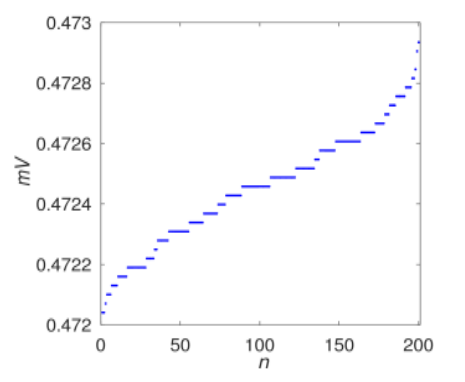
\includegraphics[scale=0.8]{../image/problem1.png}
			\end{tabular}
		\end{center}
		\caption{Исходные данные из выборки $X_1$} 
	\end{figure}

	\textbf{Диаграмма рассеяния}. Привести диаграмму рассеяния выборки с учётом погрешности прибора.
	\begin{figure}[H]
		\begin{center}
			\begin{tabular}{ccc}
				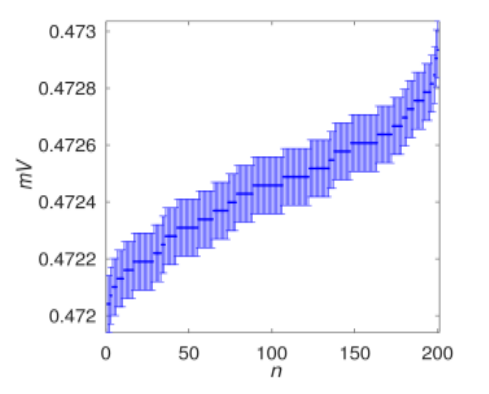
\includegraphics[scale=0.8]{../image/problem2.png}
			\end{tabular}
		\end{center}
		\caption{Диаграмма рассеяния выборки $X_1$ с уравновешенным интервалом погрешности (1)} 
	\end{figure}

	\textbf{Оценки исходной выборки}. Вычислим базовые оценки исходной выборки. Эти выборки несовместны и их информационные множества пусты. Внешние оценки найдем как
	\begin{equation}
		\underline{J} = \min_{x \leq k \leq n} \underline{x_k}, \ \overline{J} = \min_{x \leq k \leq n} \overline{x_k},
	\end{equation}
	
	Вычисления дают следующие результаты:
	\begin{equation}
		J_1 = 0.47194,\ wid J_1 = 0.47304
	\end{equation}
	Верхние и нижние вершины оценок $J_1$ совпадают с границами отображения на
	рис. 2.
	\newpage
	\section{Теория}
	Оценим выборку с помощью набора мер совместности [4].
	Сначала значения мер совместности качества возьмём в исходном, ненормированном виде:
	\begin{enumerate}
		\item Размер максимальной клики max $\mu_j$
		\item Величина коэффициента вариабельности по Оскорбину $k_0$
		\item Мера совместности Жаккара $J_i$
	\end{enumerate}
	
	Вычисление моды выборки и максимальной клики. Имеет смысл распространить понятие моды на обработку интервальных данных, где она будет обозначать интервал тех значений, которые наиболее часты, т. е. встречаются в интервалах обрабатываемых данных наиболее часто. Фактически, это означает, что точки из моды интервальной выборки накрываются наибольшим числом интервалов этой выборки. Ясно, что по самому своему определению понятие моды имеет наибольшее значение (и наибольший смысл) лишь для накрывающих выборок. Иначе, если выборка ненакрывающая, то смысл «частоты» тех или иных значений в пределах рассматриваемых интервалов этой выборки в значительной мере теряется, хотя и не обесценивается.
	
	Мода является пересечением интервалов максимальной совместной подвыборки, и если максимальных подвыборок имеется более одной, то мода будет объединением их пересечений, т. е. мультиинтервалом. Простой алгоритм вычисления моды интервальной выборки можно найти в [6]. Псевдокод специализированного алгоритма для нахождения моды выборки интервальных измерений и её частоты приведён в Табл. 1.
	
	Ключевым в алгоритме Табл. 1 является формирование множества элементарных подинтервалов измерений из упорядоченных вершин (концов интервалов) $\underline{x_1}, \overline{x_1}, \underline{x_2}, \overline{x_2}, ..., \underline{x_n}, \overline{x_n}$ исходной выборки X.
	
	Отметим также, что мода интервальной выборки — это интервал или мультиинтервал, который не обязан совпадать с каким-либо из интервалов обрабатываемой выборки.
	
	\begin{eg}
		Рассмотрим пример вычисления моды интервальной выборки
		из 4 элементов
		\begin{equation}
			X = \{[1, 4], [5, 9], [1.5, 4.5], [6, 9]\}.
		\end{equation}
	\end{eg}

	В соответствии с алгоритмом Табл. 1, проверим совместность X. Пересечение элементов выборки пусто
	\[
	\bigcap_{i = 0}^n x_i= \varnothing
	\]
	
	Таким образом, необходимо выполнить шаги алгоритма Табл. 1 после ключевого слова ELSE.
	
	Сформируем массив интервалов z из концов интервалов X
	\begin{equation}
		z = \{[1, 1.5], [1.5, 4], [4, 4.5], [4.5, 5], [5, 6], [6, 9], [9, 9]\}
	\end{equation}
	
	Для каждого интервала $z_i$ подсчитываем число $\mu_i$ интервалов из выборки X, включающих $z_i$, получаем массив значений $\mu_i$ в виде
	\begin{equation}
		\{1, 2, 1, 0, 1, 2, 2\}
	\end{equation}

	Mаксимальные $\mu_i$, равные max $\mu = 2$, достигаются для индексного множества
	\begin{center}
		$K = \{2, 6, 7\}$
	\end{center}

	Как итог, мода является мультиинтервалом
	\begin{equation}
		mode X = \bigcup_{k \in K} z_k =  [1.5, 4] \cup [6, 9] \cup [9, 9] = [1.5, 4] \cup [6, 9]
	\end{equation}

	Перейдём к практическому примеру. Проведём вычисление моды выборки $X_1$
	по алгоритму Рис. 3.

	\begin{figure}[H]
		\begin{center}
			\begin{tabular}{ccc}
				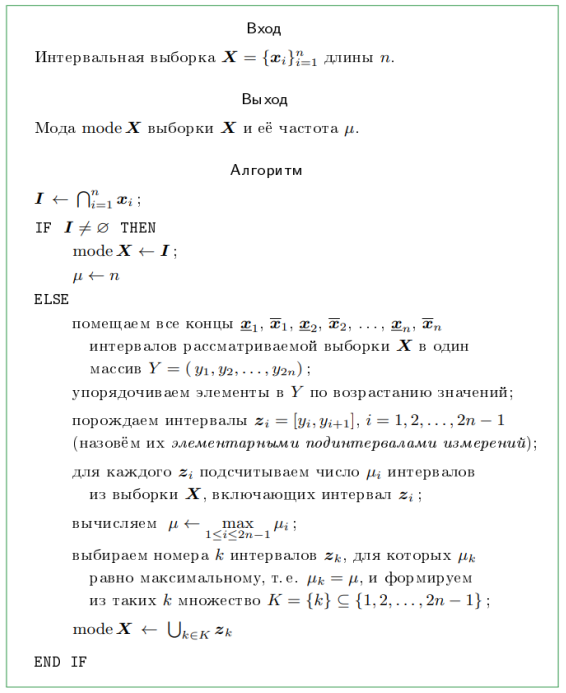
\includegraphics[scale=0.7]{../image/algorithm.png}
			\end{tabular}
		\end{center}
		\caption{Алгоритм для нахождения моды интервальной выборки} 
	\end{figure}

	\begin{figure}[H]
		\begin{center}
			\begin{tabular}{ccc}
				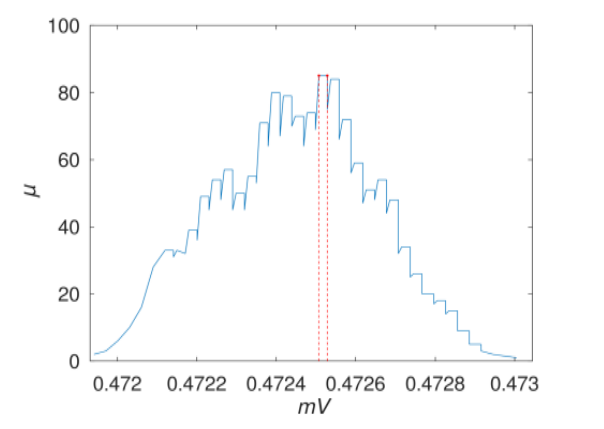
\includegraphics[scale=0.7]{../image/mu_theory.png}
			\end{tabular}
		\end{center}
		\caption{График частот при вычислении моды выборки $X_1$} 
	\end{figure}

	По результам вычисления моды выборки находим размер максимальной клики
	max $\mu_j$:
	\begin{equation}
		\max \mu_j (X_1) = 85
	\end{equation}
	Индексы таких элементов образуют множество K, а из них образуется мода
	\begin{equation}
		K = \{79, 80, ..., 163\},
	\end{equation}
	\begin{equation}
		mode X = \bigcup_{k \in K} z_k = [0.47251, 0.47253]
	\end{equation}
	На рис. 5 показаны элементы выборки $X_1$, в которые входит мода.
	
	\textbf{Варьирование неопределённости измерений}. Один из приёмов выявления достижения совместности выборки интервальных наблюдений основан на представлении о причине несовместности как недооценённой величины неопределённости [27, 28]. Закономерным шагом в этом случае становится поиск некоторой минимальной коррекции величин неопределённости интервальных наблюдений, необходимой для обеспечения совместности задачи построения зависимости. Если величину коррекции каждого интервального наблюдения $y_i = [\stackrel{o}{y_i} - \varepsilon_i, \stackrel{o}{y_i} + \varepsilon_i] = (\stackrel{o}{y_i}, \varepsilon_i)$ выборки $S_n$ выражать коэффициентом его уширения $\omega_i \geq 1$, а общее изменение выборки характеризовать суммой этих коэффициентов, то минимальная коррекция выборки в виде
	\begin{figure}[H]
		\begin{center}
			\begin{tabular}{ccc}
				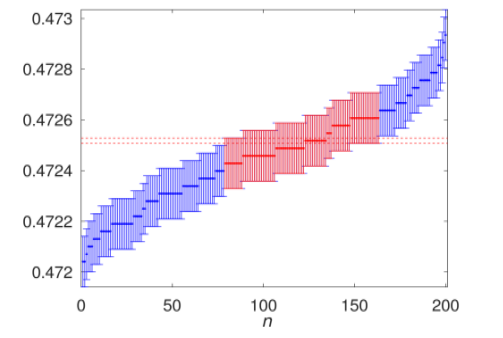
\includegraphics[scale=0.8]{../image/interval_theory.png}
			\end{tabular}
		\end{center}
		\caption{Элементы выборки $X_1$, в которые входит мода (3)} 
	\end{figure}
	
	вектора коэффициентов $\omega^* = (\omega_1^*,...,\omega_n^*)$, необходимая для совместности задачи построения зависимости $y = f(x, \beta)$ может быть найдена решением задачи условной оптимизации
	\begin{equation}
		\min_{\omega, \beta} \sum_{i=1}^{n} \omega_i
	\end{equation}
	при ограничениях
	\begin{equation}
		\begin{cases}
			\stackrel{o}{y_i} - \omega_i\varepsilon_i \leq f(x, \beta) \leq \stackrel{o}{y_i} + \omega_i\varepsilon_i\\
			\omega_i \geq 1
		\end{cases}\, i \in \overline{1,n}
	\end{equation}
	
	Результирующие значения коэффициентов $\omega_i^*$, строго превосходящие единицу, указывают на наблюдения, которые требуют уширения интервалов неопределённости для обеспечения совместности данных и модели. Именно такие наблюдения заслуживают внимания при анализе данных на выбросы. Значительное количество подобных наблюдений может говорить либо о неверно выбранной структуре зависимости, либо о том, что величины неопределённости измерений занижены во многих наблюдениях (например, в результате неверной оценки точности измерительного прибора).
	
	Следует отметить значительную гибкость языка неравенств. Он даёт возможность переформулировать и расширять систему ограничений (12) для учёта специфики данных и задачи при поиске допустимой коррекции данных, приводящей к разрешению исходной несовместности. Например, если имеются основания считать, что величина неопределённости некоторой группы наблюдений одинакова и при коррекции должна увеличиваться синхронно, то система ограничений (12) может быть пополнена равенствами вида
	\begin{equation*}
		\omega_{i_1} = \omega_{i_2} = ... = \omega_{i_K}
	\end{equation*}
	где $i_1, ..., i_K$ — номера наблюдений группы. В случае, когда в надёжности какихлибо наблюдений исследователь уверен полностью, при решении задачи (11)–(12) соответствующие им величины $\omega_i$ можно положить равными единице, т.е. запретить варьировать их неопределённость.
	
	Задача поиска коэффициентов масштабирования величины неопределённости (11)–(12) сформулирована для распространённого случая уравновешенных
	интервалов погрешности и подразумевает синхронную подвижность верхней и
	нижней границ интервалов неопределённости измерений $y_i$ при сохранении базовых значений интервалов $\stackrel{o}{y_i}$ неподвижными. При необходимости постановка задачи легко обобщается. Например, если интервалы наблюдений не уравновешены относительно базовых значений (то есть $y_i \in [\stackrel{o}{y_i} - \varepsilon_i^{-}, \stackrel{o}{y_i} + \varepsilon_i^{+}] \ \varepsilon_i^{-}\neq\varepsilon_i^{+}$ , то
	границы интервальных измерений можно варьировать независимо, масштабируя величины неопределённости $\varepsilon_i^{-}$ и $\varepsilon_i^{+}$
	с помощью отдельных коэффициентов $\omega_i^{-}$ и $\omega_i^{+}$.
	\begin{equation}
		\min_{\omega^{-}, \omega^{+}, \beta} \sum_{i=1}^{n} (\omega^{-} + \omega^{+})
	\end{equation}
	при ограничениях
	\begin{equation}
		\begin{cases}
			\stackrel{o}{y_i} - \omega_i^{-}\varepsilon_i^{-} \leq f(x_i, \beta) \leq \stackrel{o}{y_i} + \omega_i^{+}\varepsilon_i^{+}\\
			\omega_i^{-} \geq 1\\
			\omega_i^{+} \geq 1
		\end{cases}\, i \in \overline{1,n}
	\end{equation}
	Для линейной по параметрам $\beta$ зависимости $y = f(x, \beta)$ задача (11)–(12)
	представляет собою задачу линейного программирования, для решения которой
	широко доступны хорошие и апробированные программы в составе библиотек
	на различных языках программирования, в виде стандартных процедур систем компьютерной математики, а также в виде интерактивных подсистем электронных таблиц.
	
	\textbf{Оптимизация по Оскорбину}. Перейдём к практическому примеру выборки
	$X_1$. Поставим задачу линейного программирования (13) — (14) в простейшем
	виде
	\begin{equation}
		\min_{\omega, \beta} \omega
	\end{equation}
	при ограничениях
	\begin{equation}
		\begin{cases}
			\stackrel{o}{y_i} - \omega_i^{-}\varepsilon_i^{-} \leq f(x_i, \beta) \leq \stackrel{o}{y_i} + \omega_i^{+}\varepsilon_i^{+}\\
			\omega_i^{-} \geq 1\\
			\omega_i^{+} \geq 1
		\end{cases}\, i \in \overline{1,n}
	\end{equation}
	Проведём вычисление моды выборки X1 с использованием программ С.И.Жилина [8]. Синтаксис вызова программы
	
	Вычисления дают следующие результаты
	
	Оценка постоянной (18) очень близка с вычисленной ранее модой. Величина
	однородного расширения интервалов (19) достаточно велика, что соответствует
	весьма большой степени несовместности выборки $X_1$.
	На рис. 5 приведена диаграмма рассеяния выборки $X_1$ с увеличенным в $\omega$
	раз интервалом неопределённости.
	Красной пунктироной линией показана оценка постоянной (18).
	
	\textbf{Индекс Жаккара}. Для описания выборок, помимо оценок их размеров, желательно иметь дополнительную информацию о мере сходства элементов выборки. В различных областях анализа данных, биологии, информатике, в науках
	о Земле часто используют различные меры сходства множеств (см. [22]). Меру
	сходства между объектами A и B можно определить как двухместную вещественнозначную функцию $S(A, B)$, которая обладает следующими свойствами:
	
	\noindent-- ограниченность: $0 \leq S(A, B) \leq 1$;\\
	\noindent-- симметричность: $S(A, B) = S(B, F)$;
	
	\begin{figure}[H]
		\begin{center}
			\begin{tabular}{ccc}
				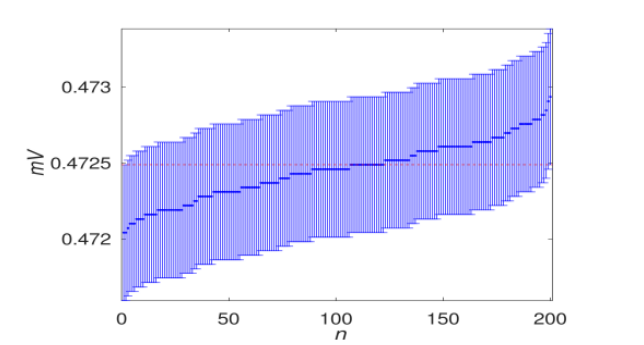
\includegraphics[scale=0.8]{../image/interval_theory_2.png}
			\end{tabular}
		\end{center}
		\caption{Диаграмма рассеяния выборки $X_1$ с увеличенным в w раз интервалом неопределённости} 
	\end{figure}

	\noindent-- неразличимость совпадающих элементов: $S(A, B) = 1 \Leftrightarrow A = B$;\\
	\noindent-- монотонность: $A \subseteq B \subseteq C \Rightarrow S(A, B) \geq S(A, C)$.
	
	Таким образом, значение 1 этой меры соответствует совпадению множеств A
	и B, а значение 0 означает их полное несходство. Отметим, что существуют
	и иные системы аксиом сходства. В компьютерных приложениях (обработка
	изображений, машинное обучение) меру сходства множеств обозначают как $I_{o}U$
	(Intersection over Union). В математике и её приложениях для подобных конструкций часто используется термин индекс Жаккара, по имени исследователя,
	впервые предложившего эту меру.
	
	В процессе развития интервального анализа были введены различные определения и конструкции оценки меры совместности интервальных объектов. Вместе с тем в практике обработки данных часто необходимо оперировать относительными величинами. В частности, это нужно в связи с необходимостью сопоставления допусков и размеров деталей, погрешности измерителей и значений
	измеряемых величин и т. п.
	
	Представим обобщение меры Жаккара на выборки интервалов [5]. В качестве
	числовой характеристики степени совпадения двух интервалов $x, y$ рассмотрим величину:
	\begin{equation}
		Ji := \frac{wid(x \wedge y)}{wid(x \vee y)}
	\end{equation}

	В выражении (20) используется ширина интервала (см. стр. ??), а вместо операций пересечения и объединения множеств — операции взятия точной нижней
	грани $1  \wedge J$ (инфимума, см. (??)) и точной верхней грани $1 \vee J$ (супремума, см. (??))
	относительно включения для двух величин в полной интервальной арифметике
	Каухера. В обозначении $J i(x, y)$ буква J указывает на фамилию «Jaccard», а
	i — на интервальность его применения. В общем случае инфимум по включению в числителе выражения (20) может быть неправильным интервалом, и его
	ширина тогда отрицательна.
	
	Рассмотренная мера обобщает обычное понятие меры совместности на различные типы взаимной совместности интервалов. Если пересечение интервалов
	x, y пусто, т. е. $x \cap y = \varnothing$, то $x \wedge y$ — неправильный интервал и числитель формулы (20) имеет отрицательное значение. В предельном случае несовпадающих
	вещественных вырожденных интервалов x = $x$ и y = $y$, $x \neq y$  имеем
	\begin{equation*}
		Ji(x,y)
	\end{equation*}
	В целом получаем
	\begin{equation}
		-1 \leq Ji(x,y) \leq 1
	\end{equation}

	Таким образом, величина $Ji$ непрерывно описывает ситуации от полной несовместности вещественных значений $x \neq y$ до полного перекрытия интервалов
	x = y. Следует заметить, что в отличие от случая вещественных величин, для
	которых индекс Жаккара может принимать только два значения, 0 и 1, формула (20) даёт характеризацию различных отношений сходства интервалов с
	помощью непрерывного ряда значений между -1 и 1.
	Мера совместности, введённая для двух интервалов в форме (20), допускает
	естественное обобщение на случай интервальной выборки $X = \{x_i\}, i = 1, 2, ..., n$.
	Определим меру $Ji(X)$ для этой выборки как
	\begin{equation}
		Ji(X) := \frac{wid(\bigwedge_{i} x_i)}{wid(\bigvee_i x_i)}
	\end{equation}
	
	Видно, что выражение (22) переходит в случае интервальной выборки из двух
	элементов в выражение (20).
	
	В связи несовместностью выборки будем использовать следующую меру, которая имеет место и в случае несовместных выборок.
	\begin{equation}
	p(mode(X)) = \frac{wid(mode(X))}{wid(\bigvee_i x_i)}	
	\end{equation}

	Назовём конструкцию (23) относительная ширина моды. В отличие от минимума по включению, мода выборки всегда является правильным интервалом. В
	целом получаем
	\begin{equation}
		0 \leq p(mode(X)) \leq 1	
	\end{equation}
	
	Вычисление меры совместности. Перейдём к практическому примеру выборки $X_1$. Проведём вычисление с использованием программ на ресурсе [23].
	\begin{equation}
		Ji(X) := \frac{wid(\bigwedge_{i} x_i)}{wid(\bigvee_i x_i)} = - 0.6344
	\end{equation}
	Отрицательность меры (25) соответствует несовместности выборки $X_1$, а её
	модуль — высокой степени этой несовместности.
	
	Относительная ширина моды (23) равна
	\begin{equation}
		p(mode(X)) = \frac{wid(mode(X))}{wid(\bigvee_i x_i)} = 0.039
	\end{equation}

	Величина (26) составляет менее $4\%$ внешней оценки выборки $X_1$.
	\section{Реализация}
	\subsection{Описание}
	Данная лабораторная работа была выполнена с использованием языка
	программирования Python 3.10 в среде разработки PyCharm с
	использованием следующих библиотек:
	\begin{itemize}
		\item math - использование математических функций
		\item matplotlib версии 3.7.1 - построение графиков
		\item numpy версии 1.24.2 - использование многомерных массивов
		\item prettytable версии 3.6.0 - вывод таблиц в консоли 
		\item scipy версии 1.10.1 - статические распределения и функции
		\item seaborn версии 0.12.2 - посроение графиков, визуализация
		\item statsmodels - дополнение к scipy, использование статистических вычислений, включая описательную статистику, оценку и вывод статистических моделей
	\end{itemize}
	Отчёт подготовлен с помощью языка LaTEX в редакторе TexStudio.
		\subsection{Ссылка на репозиторий}
		\url{https://github.com/IMZolin/Math-statistics-labs} \ - GitHub репозиторий
	
	\section{Результаты}
	\subsection{Данные выборки}
	Данные для выборки взяты из файла $Channel\_ 1\_400nm\_2mm.csv, \ \varepsilon = 10^{-4}$
	
		\begin{figure}[H]
			\begin{center}
			\begin{tabular}{ccc}
				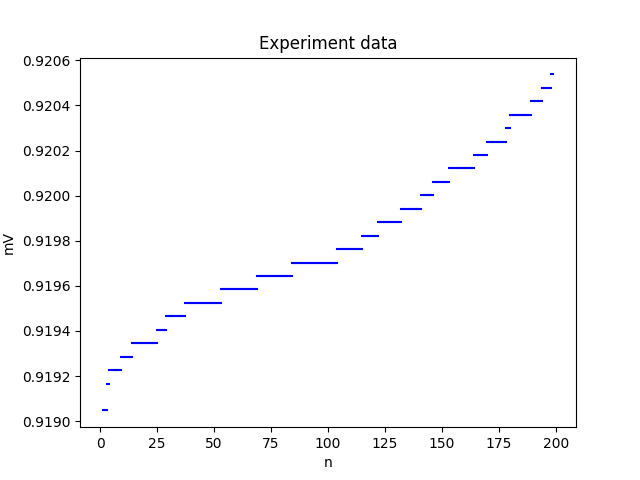
\includegraphics[scale=0.8]{../image/data.png}
			\end{tabular}
		\end{center}
			\caption{Исходные данные из выборки $X_1$} 
		\end{figure}
	 \subsection{Диаграмма рассеяния}
	\begin{figure}[H]
		\begin{center}
			\begin{tabular}{ccc}
				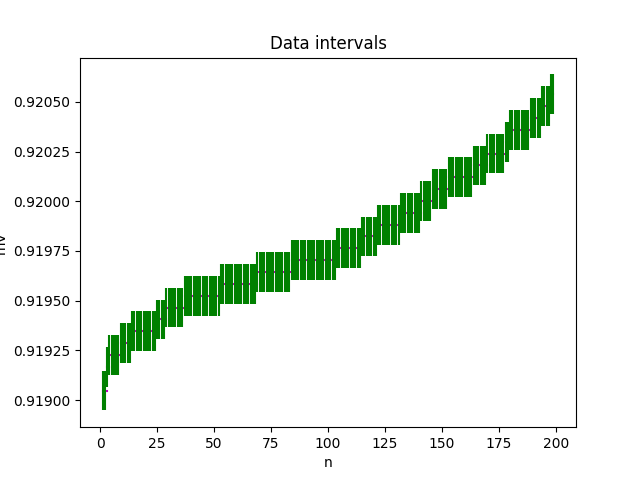
\includegraphics[scale=0.8]{../image/data_and_intervals1.png}
			\end{tabular}
		\end{center}
		\caption{Диаграмма рассеяния выборки $X_1$ с уравновешенным интервалом погрешности (1)} 
	\end{figure}

	\subsection{Оценки исходной выборки}
	\begin{center}
		$\underline{J} = \min_{x \leq k \leq n} \underline{x_k} = 0.9189881, \ \overline{J} = \min_{x \leq k \leq n} \overline{x_k} =  0.9205379,$\\
		$mid J = 0.919763, rad J = 0.000775, wid J = 0.00155.$
	\end{center}
	
	\subsection{Вычисление моды выборки и максимальной клики}
	\begin{figure}[H]
		\begin{center}
			\begin{tabular}{ccc}
				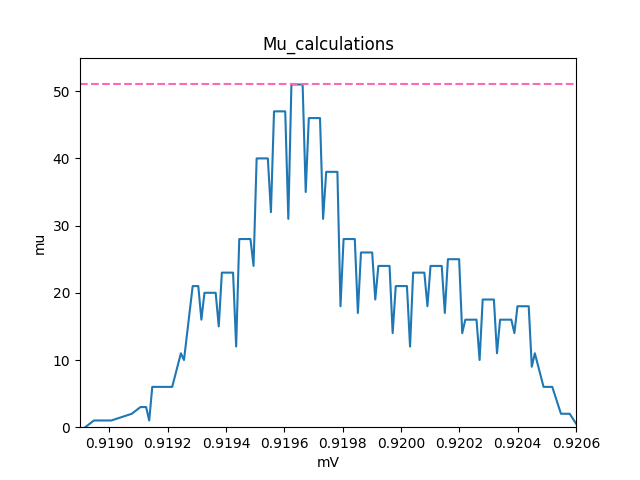
\includegraphics[scale=0.7]{../image/input_mu.png}
			\end{tabular}
		\end{center}
		\caption{График частот при вычислении моды выборки $X_1$} 
	\end{figure}

	По результам вычисления моды выборки находим размер максимальной клики max $\mu_j$:
	\begin{center}
		$\max\mu_j (X_1) = 51$
	\end{center}
	
	Индексы таких элементов образуют множество K, а из них образуется мода
	\begin{center}
		$K = {142, 143, ..., 167}$
	\end{center}
	\begin{center}
		$mode (X_1) = \bigcup_{k \in K} z_k = [0.9196246, 0.919663].$
	\end{center}
	На рис. 10 показаны элементы выборки X1, в которые входит мода.
	\begin{figure}[H]
		\begin{center}
			\begin{tabular}{ccc}
				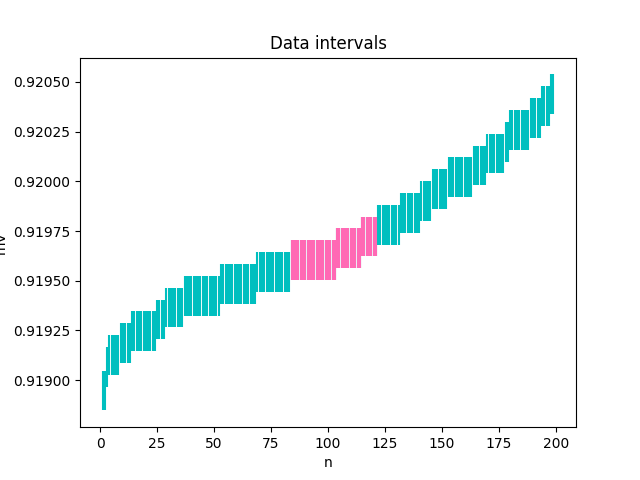
\includegraphics[scale=0.8]{../image/data_and_intervals2.png}
			\end{tabular}
		\end{center}
		\caption{Элементы выборки $X_1$, в которые входит мода (3)} 
	\end{figure}
	\subsection{Оптимизация по Оскорбину}
	Вычисления дают следующие результаты\\
	\begin{center}
		$oskorbin\_center\_k = 0.919763,$\\
		$w = 7.7490.$
	\end{center}
	На рис. 10 приведена диаграмма рассеяния выборки $X_1$ с увеличенным в w
	раз интервалом неопределённости.
	Красной линией показана оценка постоянной w.
	\begin{figure}[H]
		\begin{center}
			\begin{tabular}{ccc}
				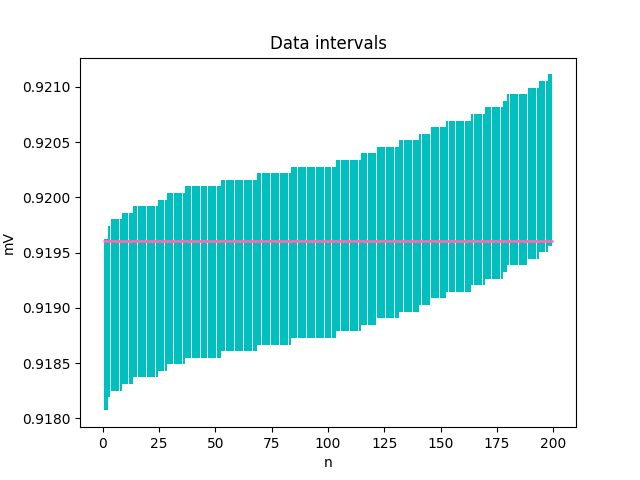
\includegraphics[scale=0.8]{../image/data_and_intervals3.png}
			\end{tabular}
		\end{center}
		\caption{ Диаграмма рассеяния выборки $X_1$ с увеличенным в w раз интервалом неопределённости} 
	\end{figure}
	\subsection{Вычисление меры совместности}
	\begin{center}
		$J_i (X) = \frac{wid(\bigwedge_{i} x_i)}{wid(\bigvee_i x_i)} = -0.77140$
	\end{center}
	Относительная ширина моды равна\\
	\begin{center}
		$p(mode(X)) = \frac{wid(mode(X))}{wid(\bigvee_i x_i)} = 0.11972$
	\end{center}
	
	
	\section{Обсуждение}
	\subsection{Оптимизация по Оскорбину}
	Оценка постоянной w близка с вычисленной ранее модой. Величина однородного расширения интервалов достаточно велика, что соответствует весьма
	большой степени несовместности выборки $X_1$.
	
	\subsection{Вычисление меры совместности}
	Отрицательность меры $J_i(X)$ соответствует несовместности выборки $X_1$, а её
	модуль — высокой степени этой несовместности.
	Абсолютное значение ширины моды зависит как от расстояния между интервалами мультивыборки, так и от ширины их максимума по включению. Величина ширины относительной моды составляет менее 12$\%$ внешней оценки выборки
	$X_1$ .
	

	\newpage
	\addcontentsline{toc}{section}{Литература}
	
	\begin{thebibliography}{4}
		\bibitem{s:hist}
		Histogram. URL: \url{https://en.wikipedia.org/wiki/Histogram}
		\bibitem{b:probSectMath}
		Вероятностные разделы математики. Учебник для бакалавров технических направлений.//Под ред. Максимова Ю.Д. --- Спб.: «Иван Федоров», 2001. --- 592 c., илл.
		\bibitem{s:boxplot}
		Box plot. URL: \url{https://en.wikipedia.org/wiki/Box_plot}
		\bibitem{a:nonParamRegr}
		Анатольев, Станислав (2009) «Непараметрическая регрессия», Квантиль, №7, стр. 37-52.
		\bibitem{a:nonParamRegr} М.З.Шварц. Данные технологических испытаний оборудования для калибровки фотоприемников солнечного излучения. 2022.
	\end{thebibliography}

\end{document}